\documentclass[25pt, a0paper, portrait, margin=0mm, innermargin=15mm, blockverticalspace=15mm, colspace=15mm, subcolspace=8mm]{tikzposter}
\usepackage{mathtools}
\usepackage[boxed]{algorithm}
\usepackage{algorithmic}
\usepackage{wrapfig}
\usepackage{pgfplots}
\usepackage{subcaption}
\usepackage{etoolbox}
\usepackage{booktabs}

\tikzposterlatexaffectionproofoff

\AtBeginEnvironment{algorithm}{%
  \setlength{\columnwidth}{\linewidth}%
}

\renewenvironment{tikzfigure}[1][]{
  \def \rememberparameter{#1}
  \vspace{10pt}
  \refstepcounter{figurecounter}
  \begin{center}
  }{
    \ifx\rememberparameter\@empty
    \else %nothing
    \\[10pt]
    %{\small Fig.~\thefigurecounter: \rememberparameter}
    {\small \rememberparameter}
    \fi
  \end{center}
}

\title{\parbox{\linewidth}{\centering Uncertainty propagation in neural networks \\ for sparse coding}}
\institute{$^{\star}$University of Sheffield, UK \quad $^{\dagger}$University of Oxford, UK }
\author{Danil Kuzin$^{\star}$, Olga Isupova$^{\dagger}$, Lyudmila Mihaylova$^{\star}$}   
\titlegraphic{
\includegraphics[width=0.25\textwidth]{graphics/University_of_Sheffield_coat_of_arms}
\vspace{-1in}
\includegraphics[width=0.247\textwidth]{graphics/oxford_coat_of_arms}}
\usetheme{Autumn}
\usecolorstyle{Britain}

\makeatletter
\renewcommand\TP@maketitle{%
    \begin{minipage}{0.2\linewidth}
       \centering
       \@titlegraphic
    \end{minipage}
    \hfill
   \begin{minipage}{0.8\linewidth}
        \centering
        \color{titlefgcolor}
        {\bfseries \Huge \sc \@title \par}
        \vspace*{1em}
        {\huge \@author \par}
        \vspace*{1em}
        {\LARGE \@institute}
    \end{minipage}%
}
\makeatother

\begin{document}
  \maketitle
  \begin{columns}
    \column{0.5}
    \block{1. LISTA}{
      \begin{minipage}[t]{0.55\linewidth}
        \vspace{0.1in}
        \coloredbox{
          Estimate \(\boldsymbol\beta \) from observations \(\mathbf{y}\) collected as \(\mathbf{y} = \mathbf{X} \boldsymbol\beta + \boldsymbol\varepsilon\), s.t.\ elements \(\boldsymbol\beta \) contain zeros. 
        }
      \end{minipage}
      \begin{minipage}[t]{0.4\linewidth}
        \begin{tikzfigure}
          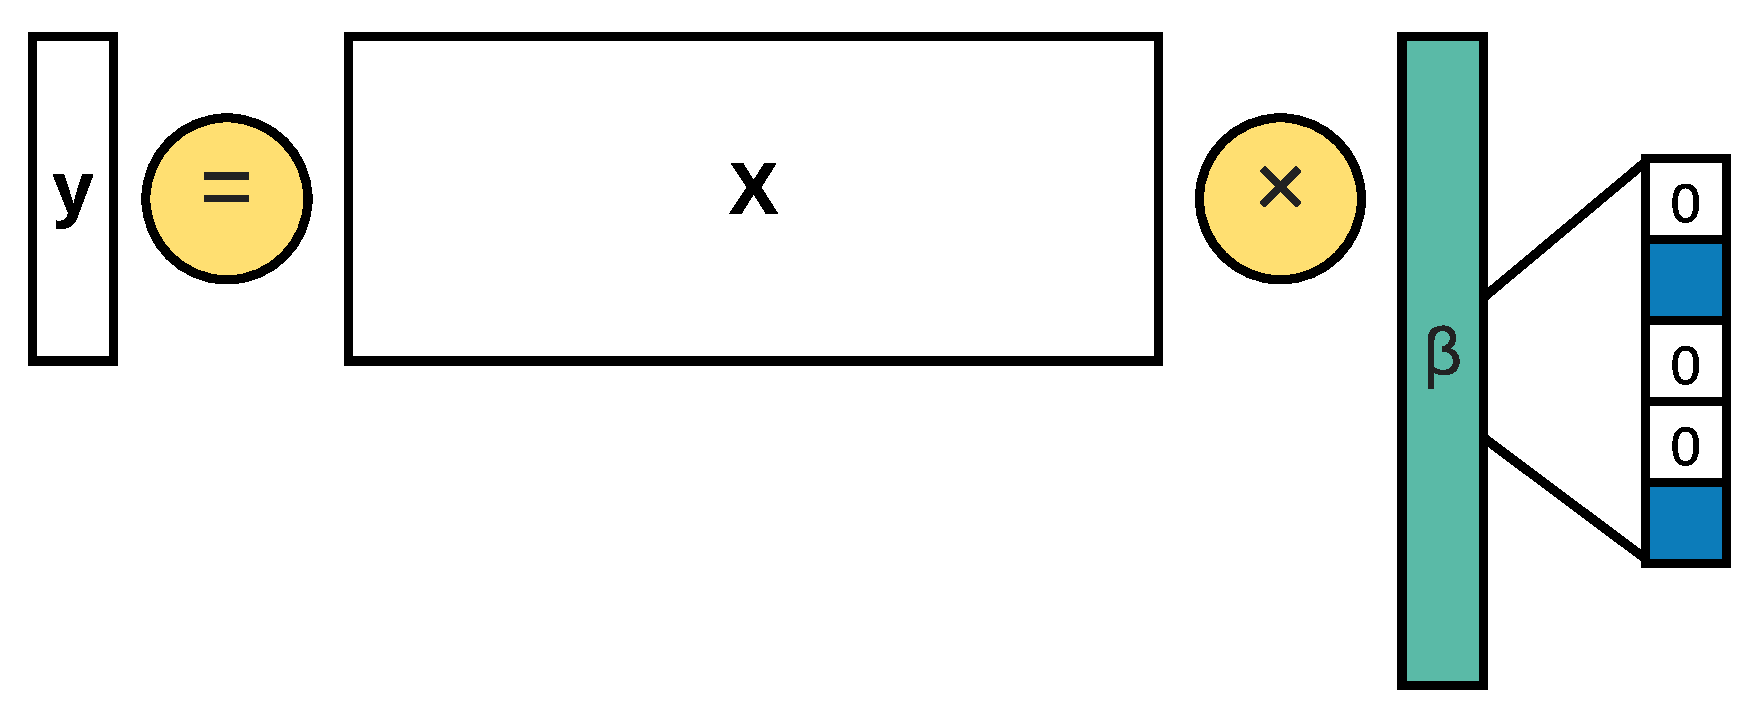
\includegraphics[width=400pt]{graphics/sparse_problem.pdf}
        \end{tikzfigure}
      \end{minipage}

      \begin{minipage}[t]{0.55\linewidth}
        \emph{LISTA} [G\&L]
        \begin{itemize}
          \item Represent iterative soft-thresholding algorithm as RNN with shared weights
          \item Learn weights with BPTT
        \end{itemize} 
      %\end{minipage}

      %\begin{minipage}[t]{0.55\linewidth}
        
        \begin{algorithm}[H]
          \begin{algorithmic}
            \STATE \textit{Init.} Dense $\mathbf{b} \gets \mathbf{W}\mathbf{y}$
            \STATE \textit{Init.} Soft-thresholding $\widehat{\boldsymbol\beta}_0 \gets h_\lambda(\mathbf{b})$
            \FOR{$l=1$ \TO $L$} 
            \STATE Dense $\mathbf{c}_l \gets \mathbf{b} + \mathbf{S}\widehat{\boldsymbol\beta}_{l-1}$
            \STATE Soft-thresholding $\widehat{\boldsymbol\beta}_{l} \gets h_\lambda(\mathbf{c}_l)$
            \ENDFOR
            \RETURN $\widehat{\boldsymbol\beta} \gets \widehat{\boldsymbol\beta}_{L}$
          \end{algorithmic}   
        \end{algorithm}
          \begin{itemize}
            \item[] {\color{red}Overfitting}
            \item[] {\color{red}No uncertainty estimation}
          \end{itemize} 
      \end{minipage} 
      \begin{minipage}[t]{0.4\linewidth} 
        \begin{tikzfigure}
          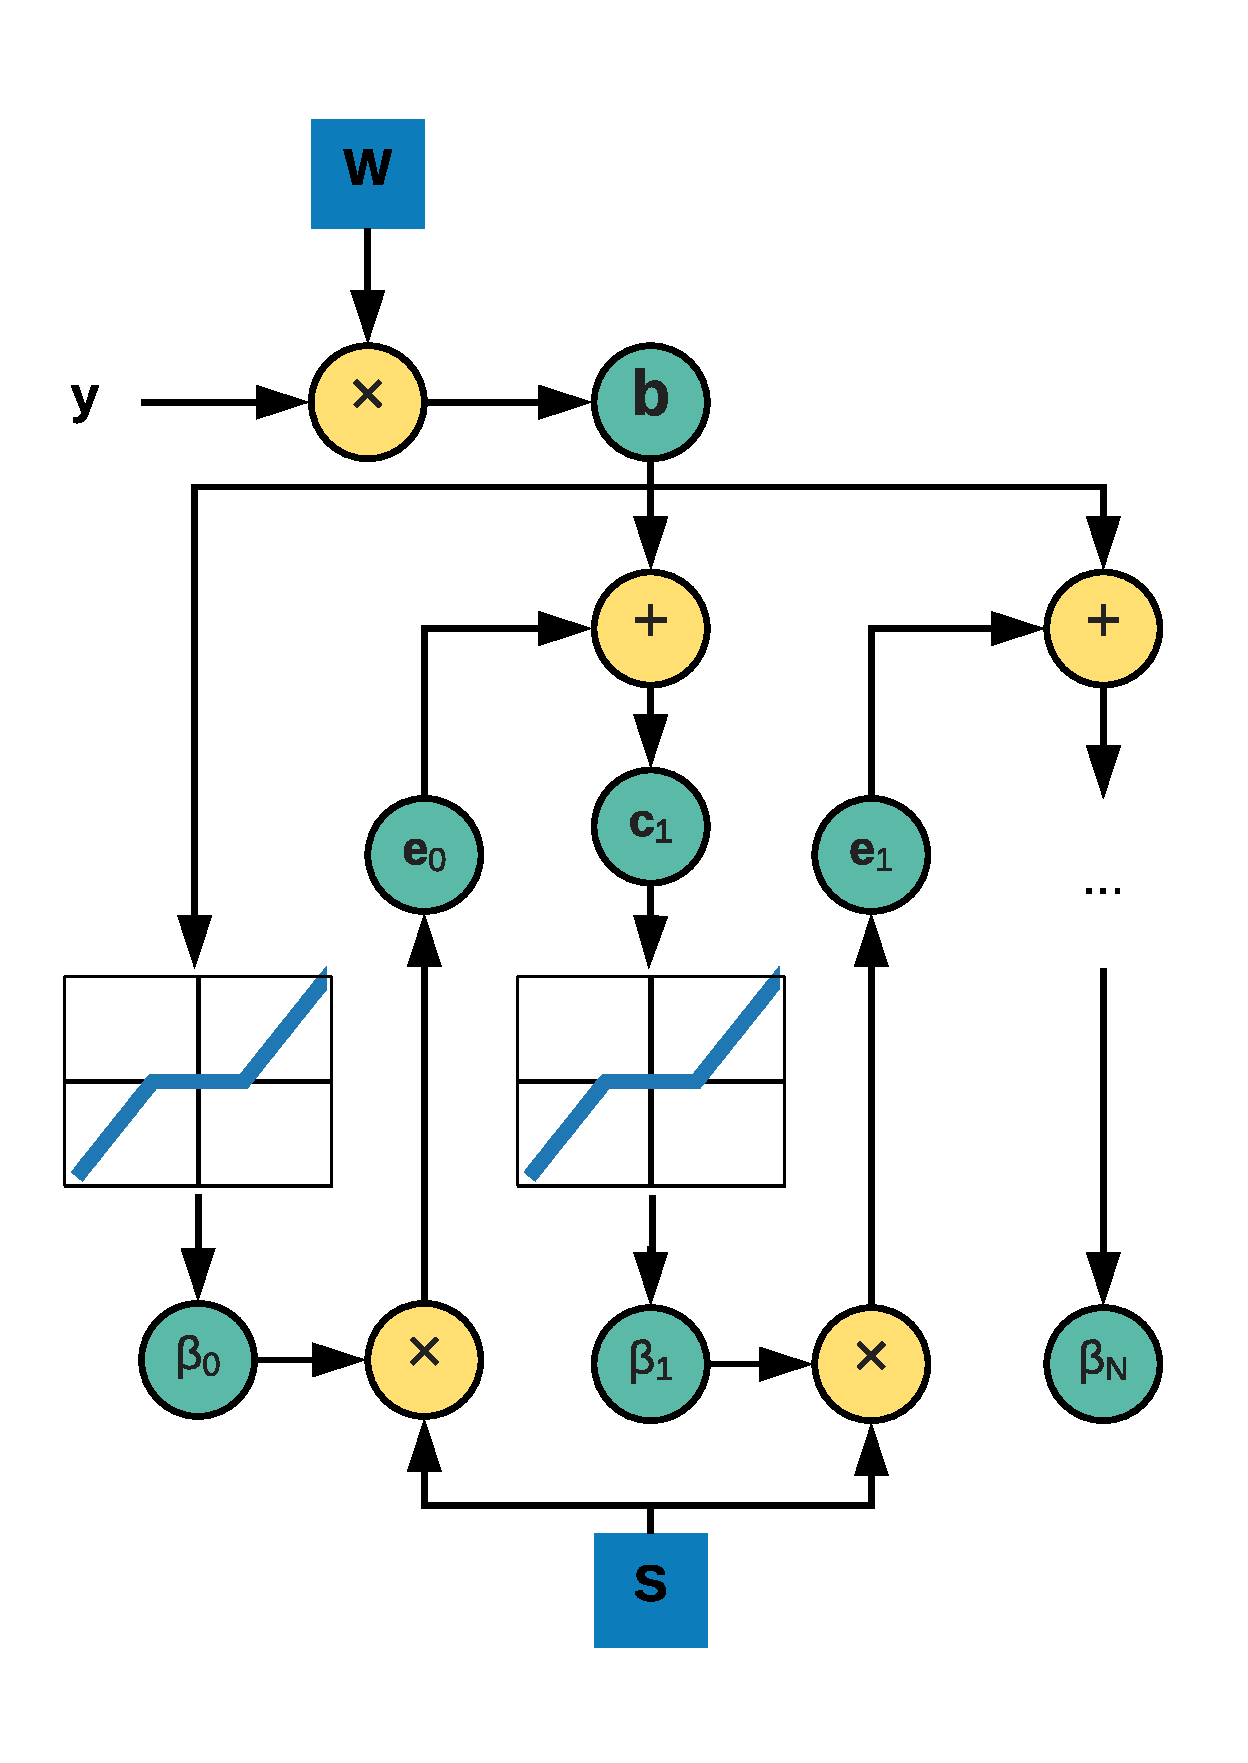
\includegraphics[width=400pt]{graphics/LISTA_main.pdf}
        \end{tikzfigure}
      \end{minipage}
    }
    \block{3. Uncertainty propagation}{
      %\innerblock{Idea}{
        At every step the output of soft-thresholding can be closely approximated with the spike and slab distribution
      \begin{enumerate}
        \item \(\mathbf{b} = \mathbf{W}\mathbf{y}\) is Gaussian-distributed
        \begin{tikzfigure}
          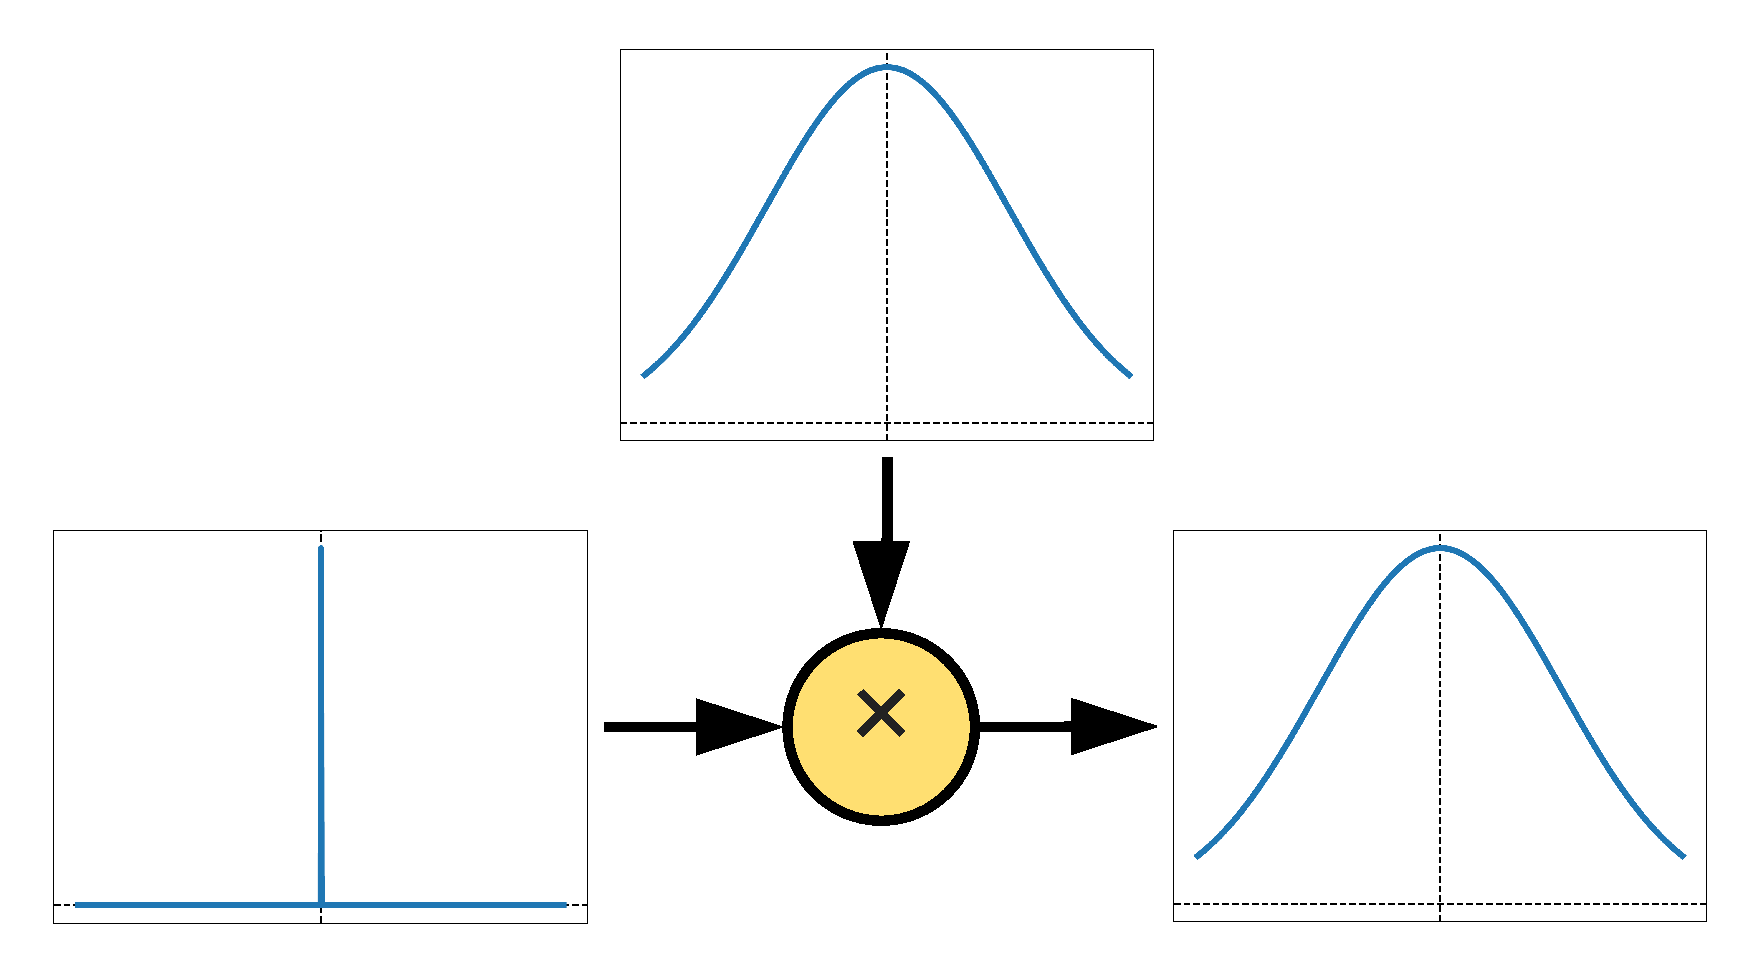
\includegraphics[width=440pt]{graphics/gauss_delta.pdf}
        \end{tikzfigure}
        \item \(\widehat{\boldsymbol\beta}_{0} = h_\lambda(\mathbf{b})\) is approximated with the spike and slab distribution
        \begin{tikzfigure}
          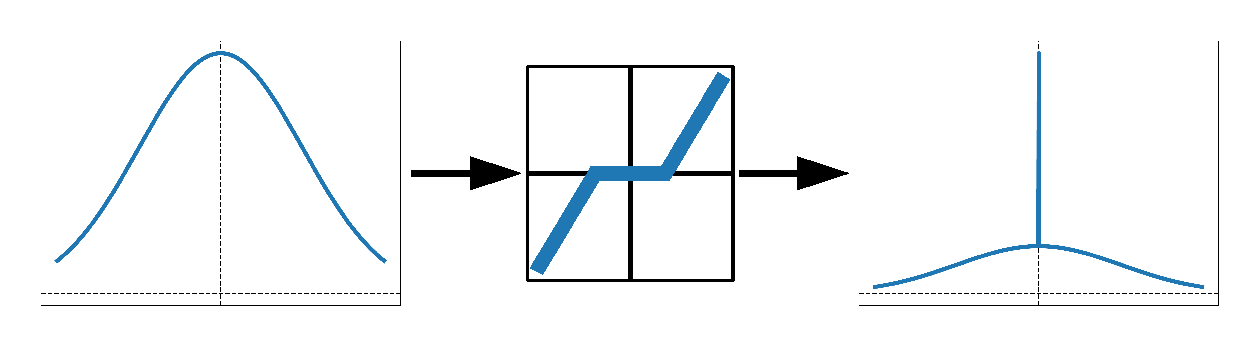
\includegraphics[width=440pt]{graphics/spsl_propagation.pdf}
        \end{tikzfigure}
        \item \(\mathbf{e}_l = \mathbf{S}\widehat{\boldsymbol\beta}_{l-1}\) is approximated with the Gaussian distribution
        \begin{tikzfigure}
          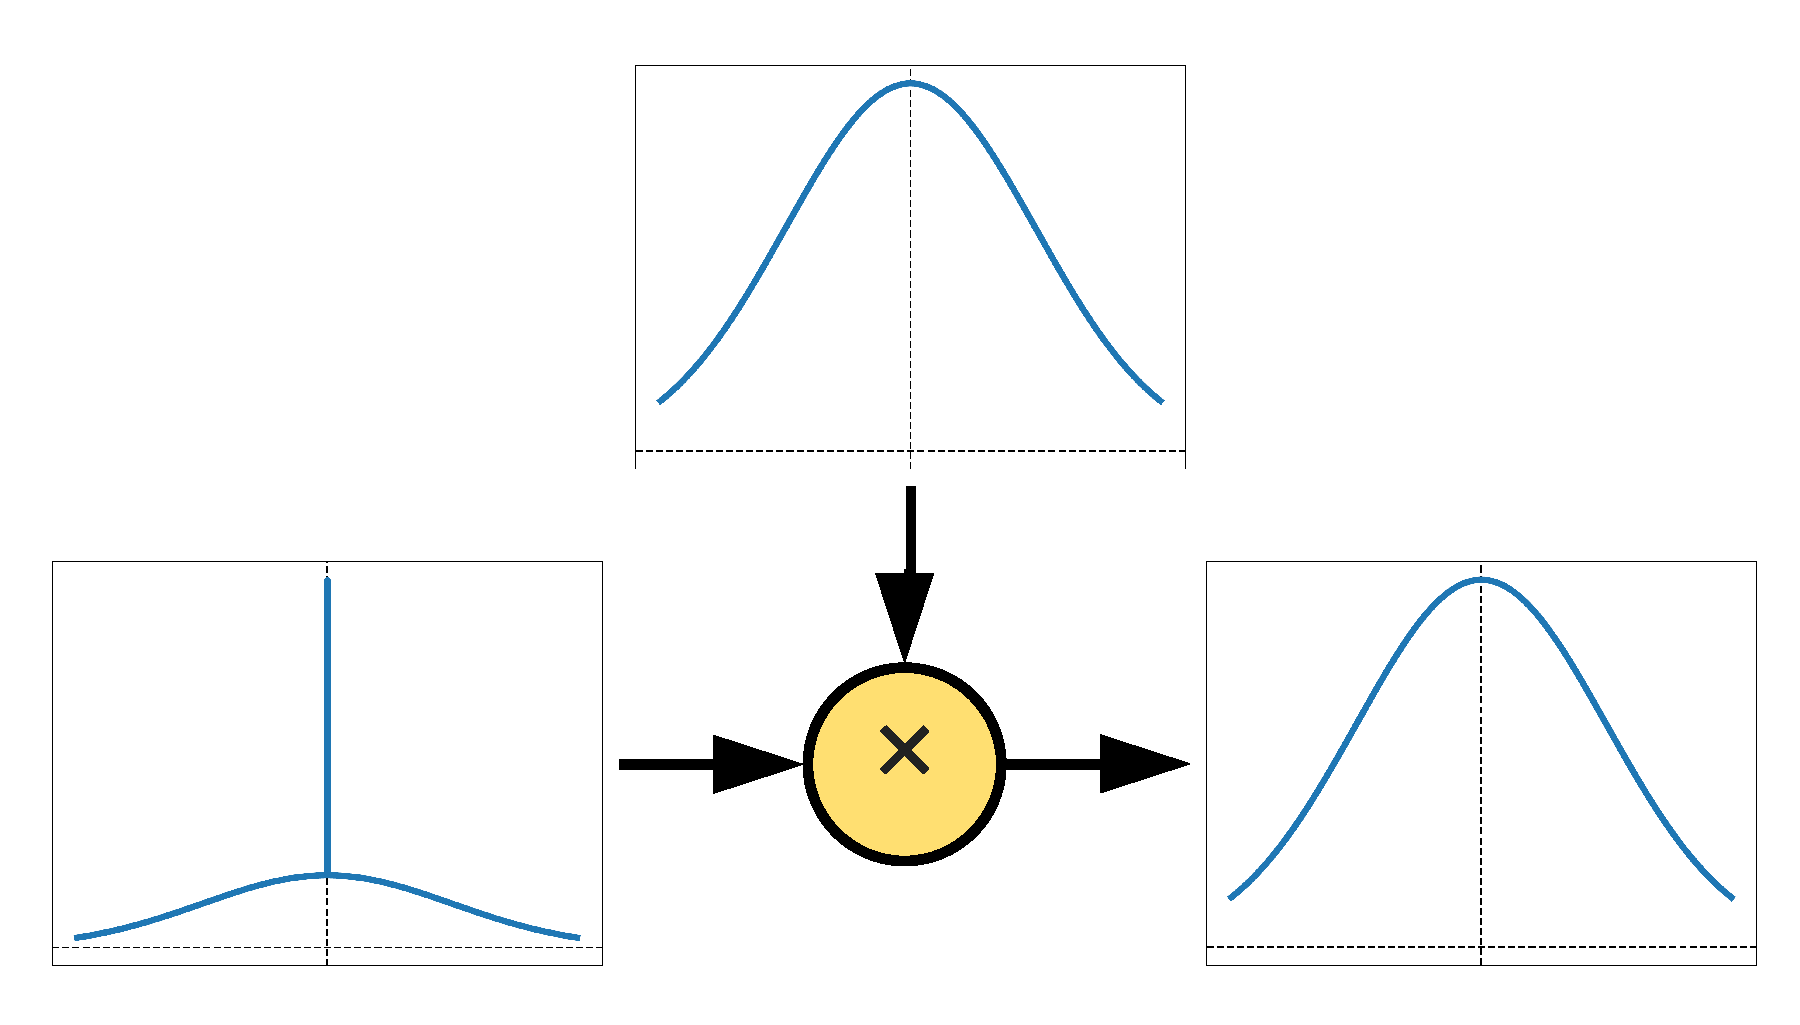
\includegraphics[width=440pt]{graphics/gauss_spsl.pdf}
        \end{tikzfigure}
        \item \(\mathbf{c}_l = \mathbf{b} + \mathbf{e}_l\) is Gaussian-distributed
        \begin{tikzfigure}
          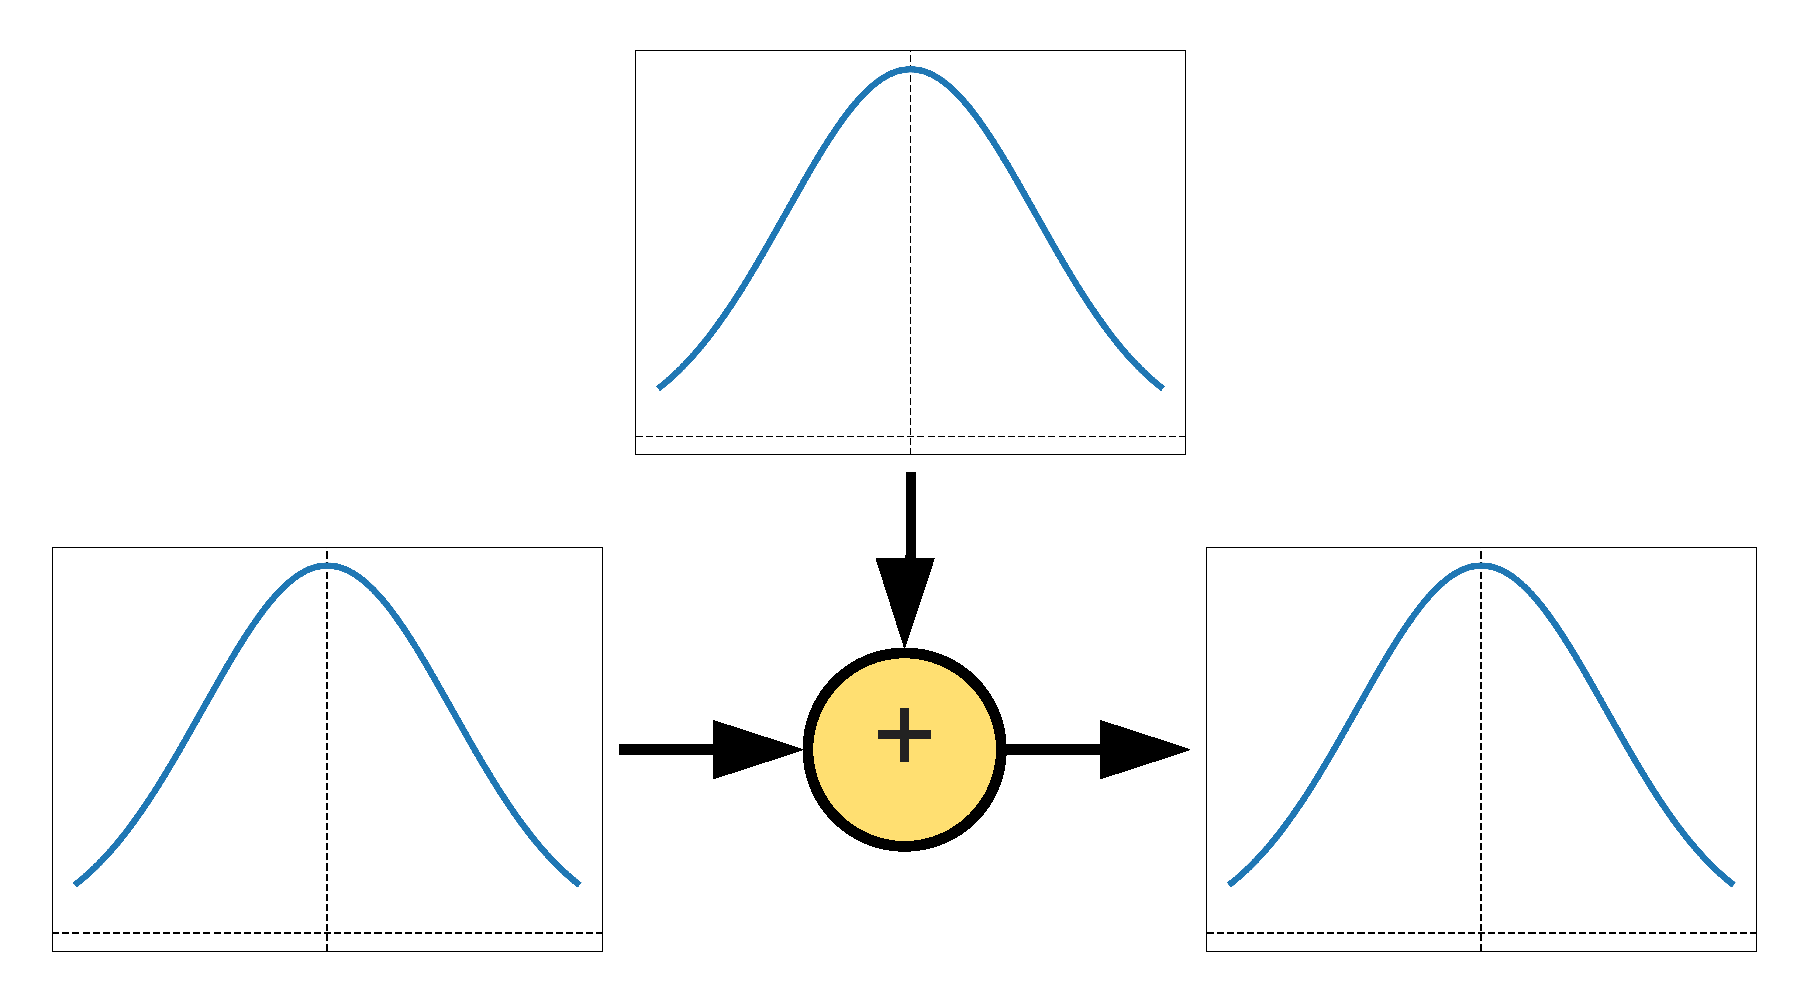
\includegraphics[width=440pt]{graphics/gauss_gauss.pdf}
        \end{tikzfigure}
        \item \(\widehat{\boldsymbol\beta}_{l} = h_\lambda(\mathbf{c}_l)\) is approximated with the spike and slab distribution
        \begin{tikzfigure}
          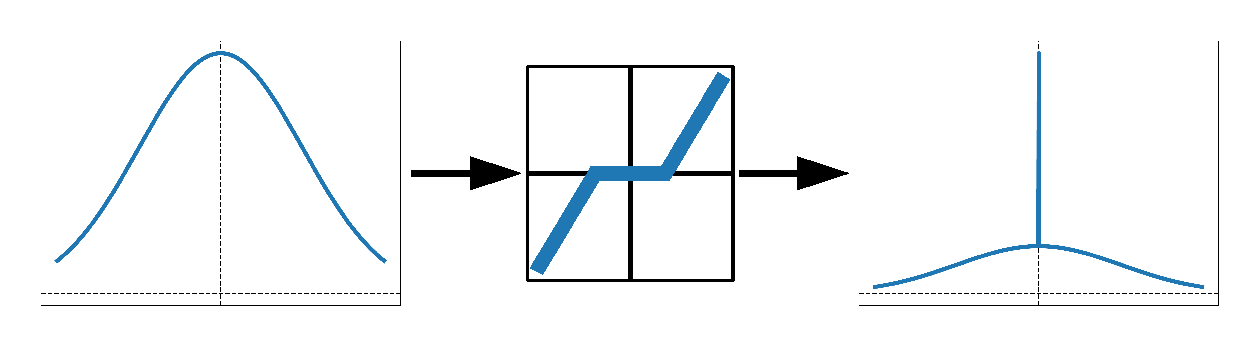
\includegraphics[width=440pt]{graphics/spsl_propagation.pdf}
        \end{tikzfigure}
    \end{enumerate}
      %}
      %\innerblock{Advantages}{
        \begin{itemize}
          \item[] {\color{blue}All latent variables are modelled with parametrised distributions}
          \item[] {\color{blue}We can apply approximate Bayesian inference methods}
        \end{itemize}
      %}
    }
    \block{6. References}{
      \begin{itemize}
        \item[] [HL\&A] J. M. Hern{\'a}ndez-Lobato, R. Adams. Probabilistic backpropagation for scalable learning of Bayesian neural networks. ICML 2015.
        \item[] [G\&L] K. Gregor, Y. LeCun. Learning fast approximations of sparse coding. ICML 2010.
      \end{itemize}
    }
    \column{0.5}
    \block{2. BayesLISTA}{ 
      \begin{itemize}
        \item Add priors for NN weights
        \begin{equation*}
          p(\mathbf{W}) = \prod_{d=1}^D\prod_{k=1}^K \mathcal{N}(w_{ij} ; 0, \eta^{-1}), \quad
          p(\mathbf{S}) = \prod_{d'=1}^D\prod_{d''=1}^D \mathcal{N}(s_{d'd''} ; 0, \eta^{-1}),
        \end{equation*}
        \item Propagate distribution for $\widehat{\boldsymbol\beta}$ through layers
        \item Compute prediction as noisy NN output
        \begin{equation*}
          p(\mathbf{\boldsymbol\beta}| \mathbf{y}, \mathbf{W}, \mathbf{S}, \gamma, \lambda)
          = \prod_{d=1}^D\mathcal{N}\left(\beta_d; [f(\mathbf{y} ; \mathbf{S}, \mathbf{W}, \lambda)]_d, \gamma^{-1}\right)
        \end{equation*}
        \item Update weights with PBP
      \end{itemize}
      }
    \block{4. BackProp-PBP}{
      Approximate posterior
    \begin{align*}
    \label{eq:approximating_dsitribution}
    \begin{split}
    q(\mathbf{W}, \mathbf{S}, \gamma, \eta) &= \prod_{d=1}^D\prod_{k=1}^K \mathcal{N}(w_{dk} ; m^w_{dk}, v^w_{dk}) \prod_{d'=1}^D\prod_{d''=1}^D \mathcal{N}(s_{d'd''} ; m^s_{d'd''}, v^s_{d'd''}) \\
    &\times \text{Gam}(\gamma; a^\gamma, b^\gamma) \text{Gam}(\eta; a^\eta, b^\eta)
    \end{split}
    \end{align*}
    
    \coloredbox{
      Probabilistic backpropagation [HL\&A]: use derivatives of the logarithm of a normalisation constant to update weight distributions
    }
    \begin{equation*}
    q(a) = Z^{-1}f(a)\mathcal{N}(a; m, v)
    \end{equation*}
    \begin{equation*}
    Z \approx \prod_{d=1}^D \left[\omega^{\widehat{\boldsymbol\beta}}_d  \mathcal{T}\left(\beta_d ; 0, \beta^\gamma / \alpha^\gamma, 2\alpha^\gamma\right) + \vphantom{m^{\widehat{\boldsymbol\beta}}_d} \left(1 - \omega^{\widehat{\boldsymbol\beta}}_d\right)\mathcal{N}\left(\beta_d ; m^{\widehat{\boldsymbol\beta}}_d,  \beta^\gamma / (\alpha^\gamma - 1) + v^{\widehat{\boldsymbol\beta}}_d\right)\right],
    \end{equation*}
    where $\{\omega^{\widehat{\boldsymbol\beta}}_d, m^{\widehat{\boldsymbol\beta}}_d, v^{\widehat{\boldsymbol\beta}}_d\}$ are the parameters of the spike and slab distribution for $[\widehat{\boldsymbol\beta}]_d$. 
    
    }
    \block{5. Results}{
      %\innerblock{Synthetic Experiments}{
        \emph{Synthetic}
        \begin{tikzfigure}[Different depth performance]
                     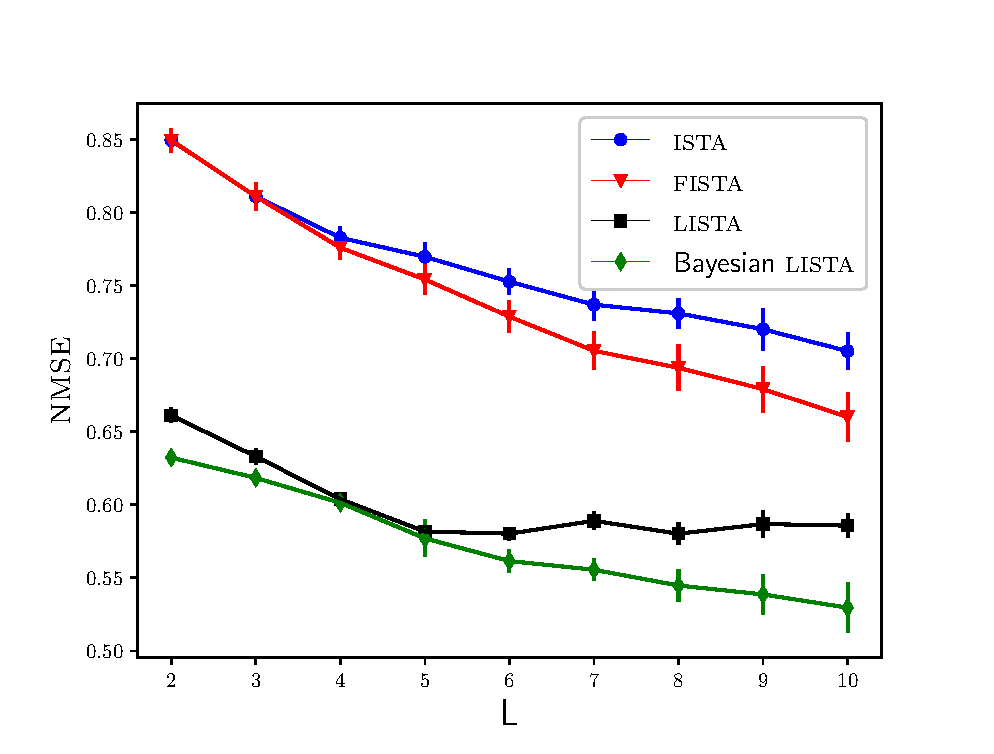
\includegraphics[width=300pt]{graphics/synthetic_number_of_layers/nmse_validation}
\quad
                     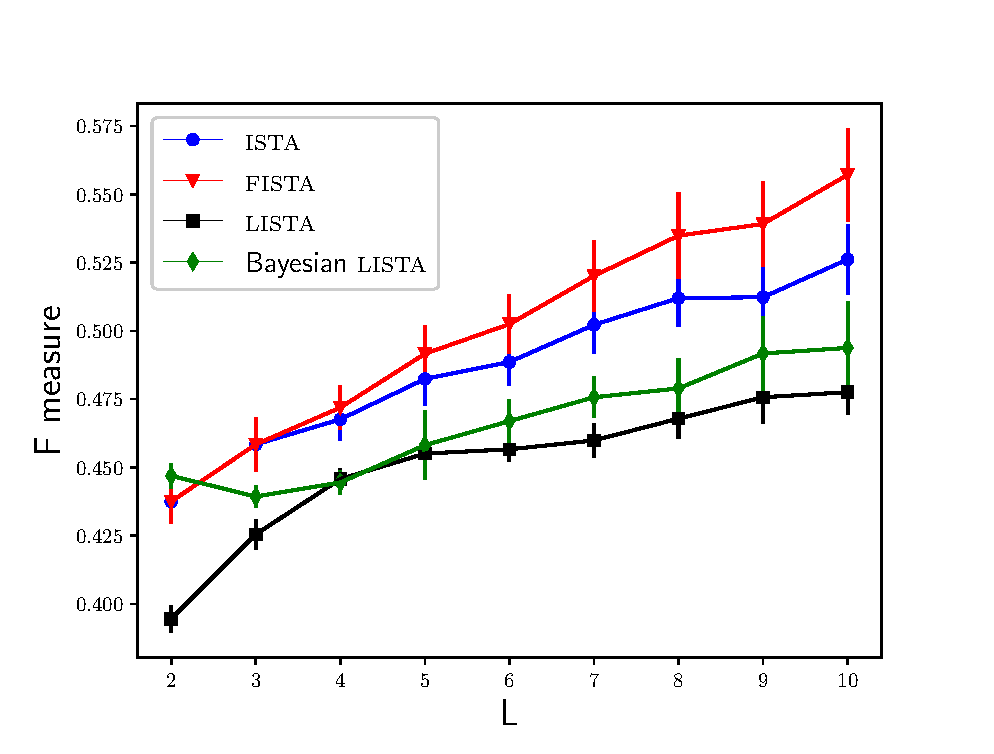
\includegraphics[width=300pt]{graphics/synthetic_number_of_layers/f_measure_validation}
          %\captionsetup{labelformat=empty}
        \end{tikzfigure}

        \begin{tikzfigure}[Different observation size performance]
                     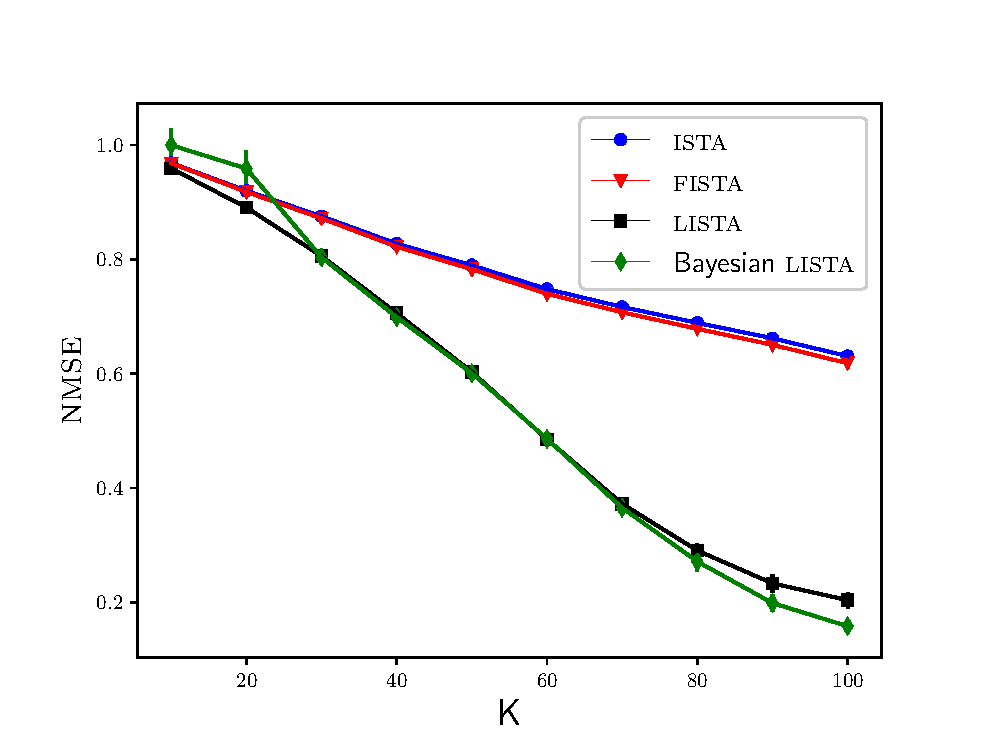
\includegraphics[width=300pt]{graphics/synthetic_undersampling/nmse_validation}
          \quad
                     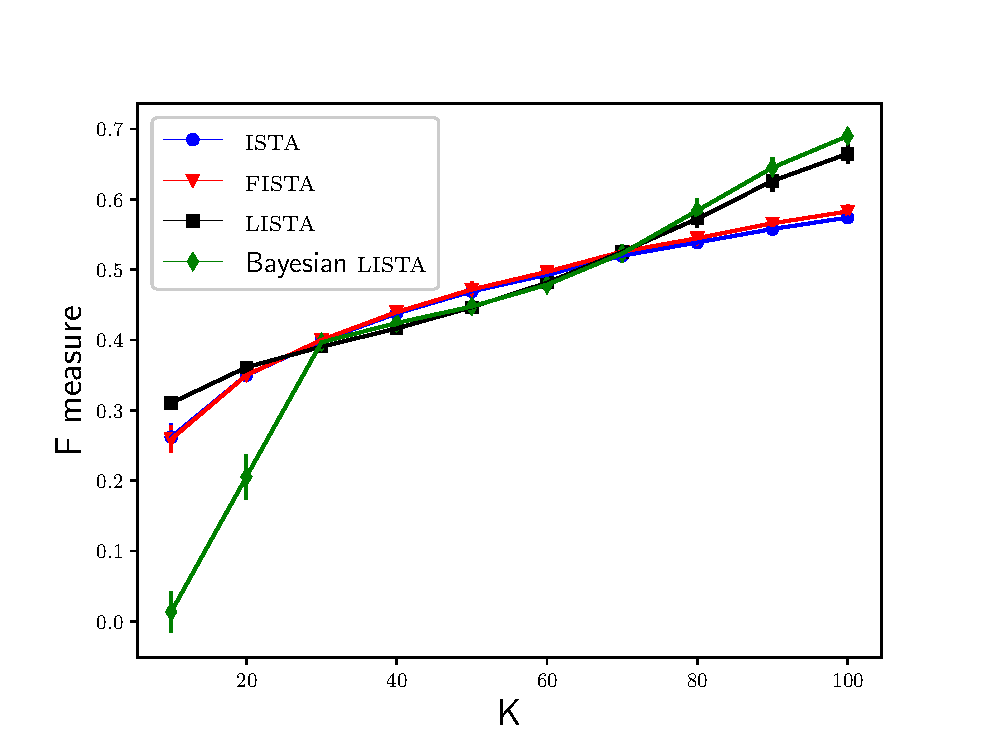
\includegraphics[width=300pt]{graphics/synthetic_undersampling/f_measure_validation}
          %\captionsetup{labelformat=empty}
        \end{tikzfigure}
      %}
      \emph{MNIST}
      %\innerblock{MNIST Experiments}{
        \begin{tikzfigure}[Posterior mean and spike indicator for an image of digit 7]
            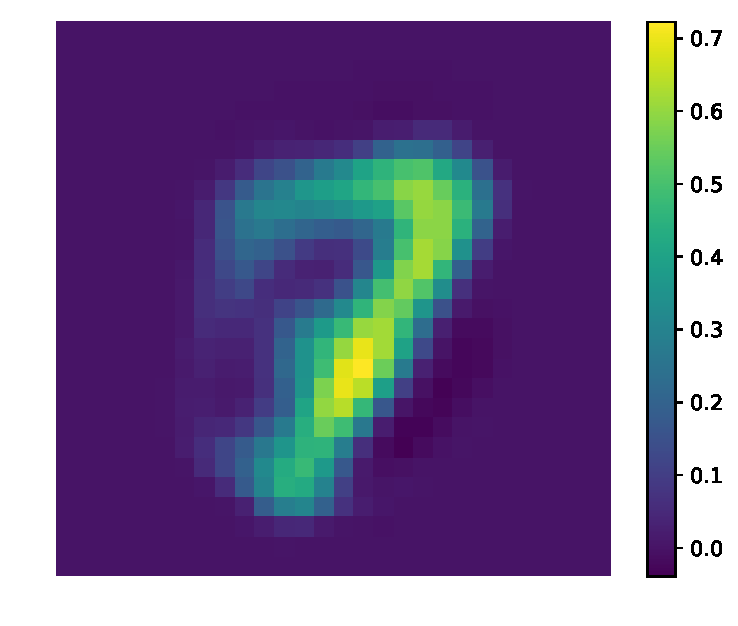
\includegraphics[width=200pt]{graphics/posterior_mean}
          \quad
            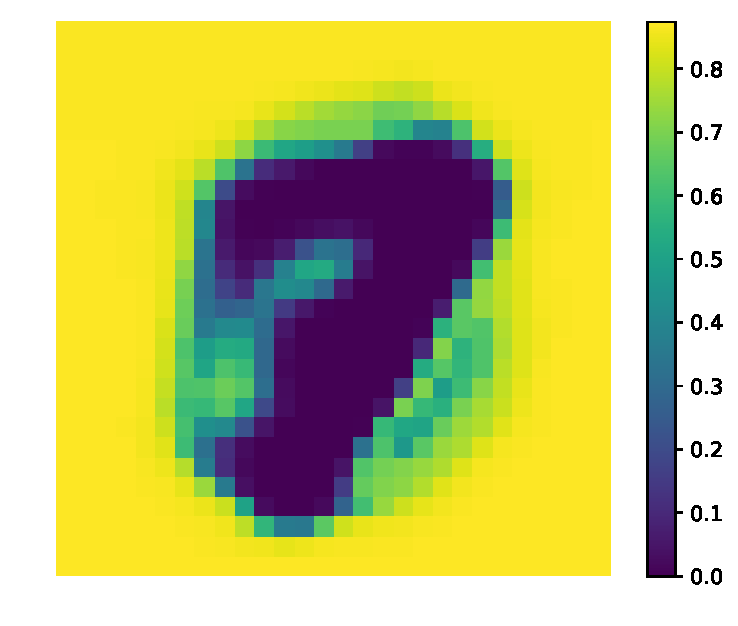
\includegraphics[width=200pt]{graphics/posterior_spike_indicator}
        \end{tikzfigure}

        \begin{tikzfigure}[Samples from the posterior for an image of digit 7]
            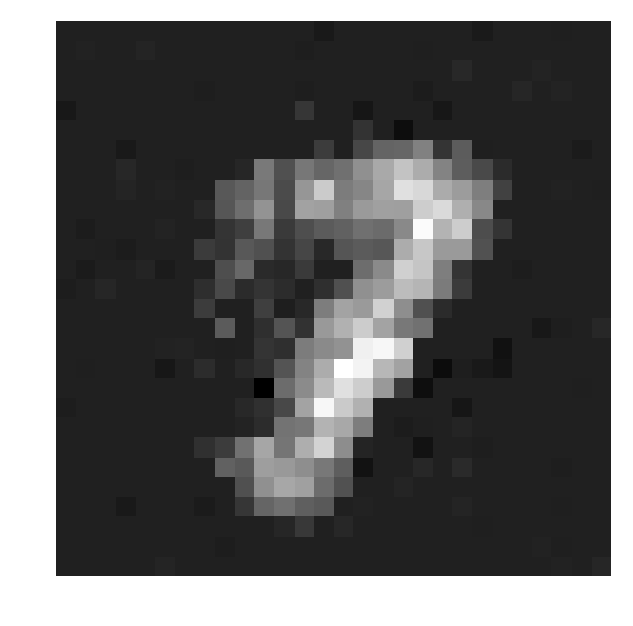
\includegraphics[width=200pt]{graphics/posterior_sample_0}
          \quad
            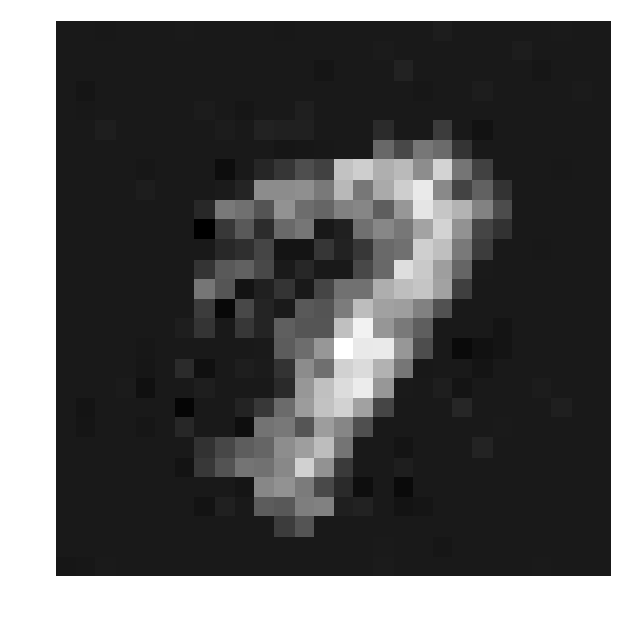
\includegraphics[width=200pt]{graphics/posterior_sample_1}
          \quad
            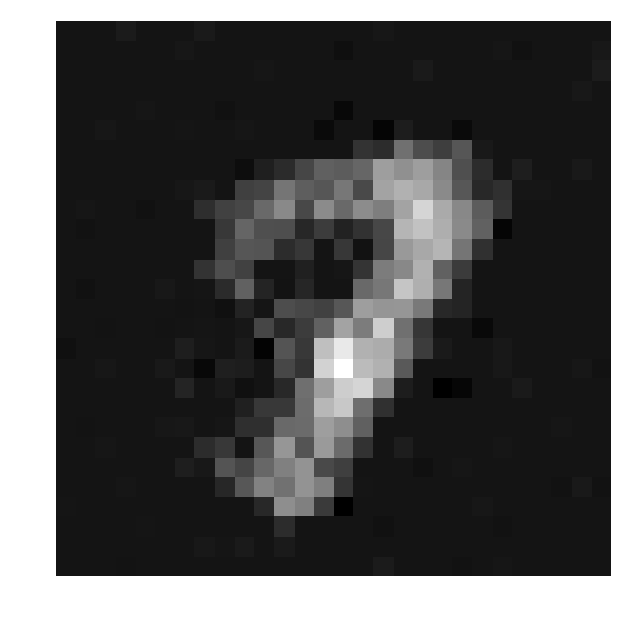
\includegraphics[width=200pt]{graphics/posterior_sample_2}
        \end{tikzfigure}
      %}
      
      %\innerblock{Active Learning}{
      \emph{Active Learning}
        Use the estimated uncertainty to choose next training data with largest variance
        \begin{tikzfigure}[Sequential pool additions]
            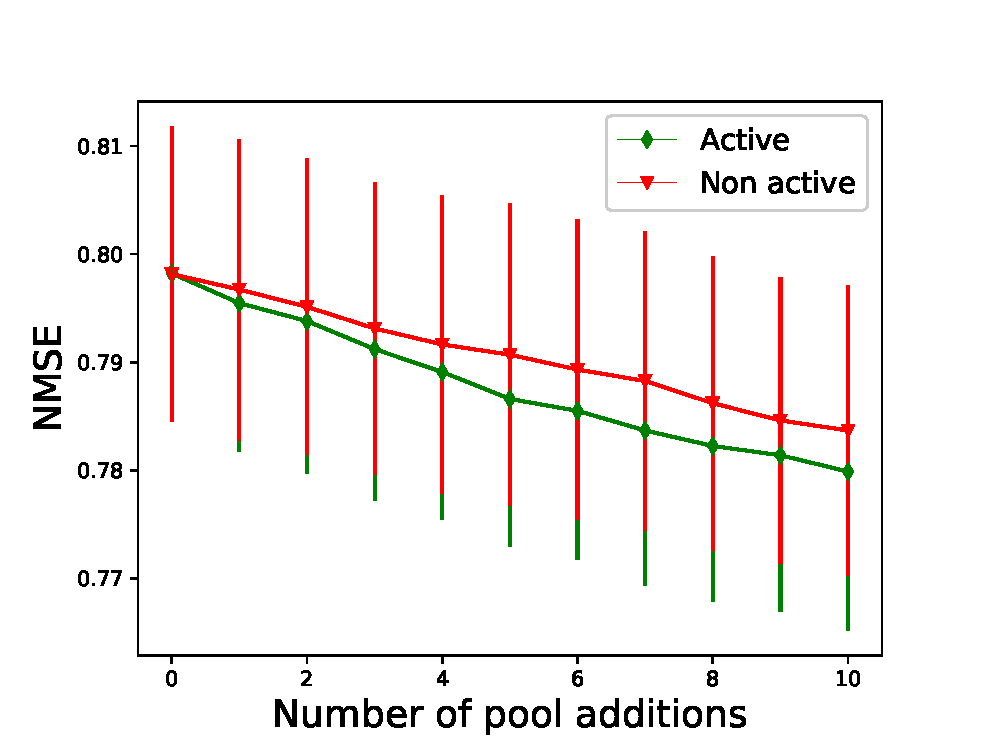
\includegraphics[width=300pt]{graphics/active_mnist/nmse_validation}
            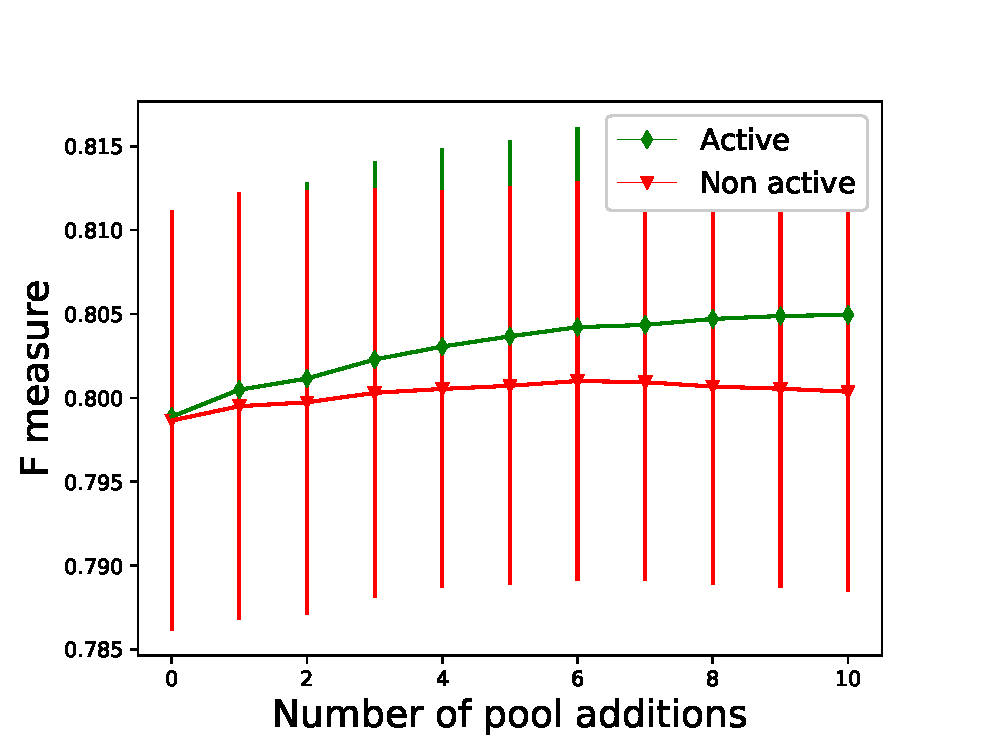
\includegraphics[width=300pt]{graphics/active_mnist/f_measure_validation}
        \end{tikzfigure}
      %}


    }
  \end{columns}
\end{document}
